\setAuthor{Tundmatu autor}
\setRound{lahtine}
\setYear{2005}
\setNumber{G 3}
\setDifficulty{3}
\setTopic{Staatika}

\prob{Kuul}
Metallist kuul asetseb lauaaugus, mille sügavus on 2 korda väiksem kuuli raadiusest (vt joonist). Kui suure laua kaldenurga $\alpha$ puhul kukub kuul august välja? 

\begin{center}
	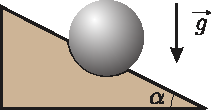
\includegraphics[width=0.4\linewidth]{2005-lahg-03-yl}
\end{center}

\hint
Kuuli hoiab augus või \enquote{lükkab} august välja üks ja sama jõud --- kuulile mõjuv raskusjõud, mis on suunatud vertikaalselt alla. Kuul on augus, kui raskusjõu vektor läbib augu põhja, ja kukub, kui see väljub sellest.

\solu
Kuuli hoiab augus või \enquote{lükkab} august välja üks ja sama jõud --- kuulile mõjuv raskusjõud, mis on suunatud vertikaalselt alla. Kuul on augus, kui raskusjõu vektor läbib augu põhja, ja kukub, kui see väljub sellest. Esimesel juhul on raskusjõu moment suunatud augu poole, teisel juhul august välja. Piirjuhul on kuul tasakaalus, toetudes vaid punktile $A$ (vt joonist). Sellel juhul on kuulile mõjuv raskusjõud suunatud otse punkti $A$ poole, jõuõlg ning järelikult ka jõumoment on võrdne nulliga.

Vaatleme piirjuhtu (vt joonist). Kuna lauaaugu sugavus $|BC|$ on 2 korda väiksem, kui kuuli raadius $r$, saame kolmnurga $AOB$ kohta kirjutada järgneva tingimuse:
\[
\sin \gamma=\frac{r / 2}{r}=\frac{1}{2} \quad \Rightarrow \quad \gamma=\arcsin \frac{1}{2}=\ang{30}.
\]
Kuna punkti $A$ tipunurgad on võrdsed, siis ka täisnurkse kolmnurga $ADE$ üksnurkadest on \ang{30}. Järelikult
\[
\alpha = \ang{90} - \ang{30} = \ang{60}.
\]
Kui laua kaldenurk ületab \ang{60}, kukub kuul lauaaugust välja.
\begin{center}
	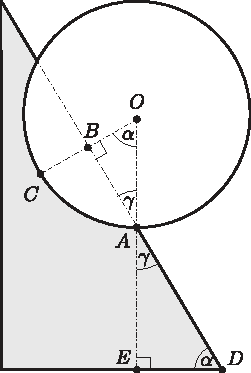
\includegraphics[width=0.35\linewidth]{2005-lahg-03-lah}
\end{center}
\probend